\documentclass{BeamerTemplate}

\usepgfplotslibrary{statistics}
\pgfplotsset{compat=1.17}

% Couleurs des groupes (A, B) pour les graphiques
\definecolor{grA}{HTML}{F8766D}
\definecolor{grB}{HTML}{00BFC4}
\definecolor{grC}{HTML}{7CAE00}

% Style commun des petits diagrammes en points
\pgfplotsset{
  pointsANOVA/.style={
    width=4.3cm, height=5.2cm,
    ymin=2, ymax=24, ytick={5,10,15,20},
    xmin=0.4, xmax=2.6,
    axis lines=left, tick label style={font=\scriptsize},
    ymajorgrids, grid style={black!10},
    title style={font=\small},
  }
}

\title{Chapitre 5a -- Analyse de la variance}
\subtitle{STT-1920 Méthodes statistiques}
\date{}

\begin{document}
\begin{frame}[t]
  \titlepage
\end{frame}

%-------------------------------------------------------------------------------
\section{Introduction}
%-------------------------------------------------------------------------------

\begin{frame}[t]{Objectifs de l'analyse de la variance (ANOVA)}

\begin{Boite}{Analyse de la variance à un facteur}
\begin{itemize}
  \item Comparer les \alert{moyennes} d'une variable dans \alert{plusieurs populations}
  (normales, de même variance);
  \item Déterminer si un \alert{facteur} (variable discrète ou qualitative) a une
  influence sur une \alert{variable réponse} (variable aléatoire continue).
\end{itemize}
\end{Boite}

\end{frame}

\begin{frame}[t]{Exemples}

\begin{itemize}\itemsep3mm
  \item Un ingénieur aux transports veut comparer la durabilité moyenne de
  7 mélanges de peinture pour asphalte.
  \item<2-> Un chercheur développe 3 traitements contre l'hypertension. Il désire
  savoir si l'un d'entre eux a un délai d'action plus court que les autres.
  \item<3-> Un agronome veut savoir si les 4 variétés de blé qui résistent le mieux
  à la moisissure donnent des rendements moyens égaux.
  \item<4-> Un directeur de magasin d'appareils électroniques veut comparer
  5 méthodes de publicité: sont-elles équivalentes ou l'une d'elles
  amène-t-elle plus de clients que les autres?
\end{itemize}

\end{frame}

%-------------------------------------------------------------------------------
\section{Principes d'expérimentation}
%-------------------------------------------------------------------------------

\begin{frame}[t]{Pourquoi planifier une expérience?}

Pour qu'une expérience mène à une conclusion fiable,
\begin{enumerate}
  \item elle doit être \alert{bien planifiée};
  \item ses résultats doivent être \alert{adéquatement analysés} (c'est l'ANOVA).
\end{enumerate}
On planifie pour se protéger contre les \alert{biais} et pour \alert{contrôler la
variabilité} due à d'autres facteurs que celui qui nous intéresse.

\begin{Boite}{Exemple 1: régimes alimentaires chez la souris}
\small
Une chercheuse veut savoir si trois régimes (standard, riche en gras, riche en
fibres) mènent au même \alert{gain de poids} moyen chez la souris après 8 semaines.
Elle dispose de 24 souris, chacune logée dans sa propre cage.
\end{Boite}

\uncover<2->{\small Or, le gain de poids varie aussi selon le poids initial, l'âge,
le sexe, la portée d'origine, l'emplacement de la cage (température, lumière), la
personne qui manipule les souris\ldots\ \alert{Comment isoler l'effet du régime?}}

\end{frame}

\begin{frame}[t]{Trois principes essentiels}

\begin{Boite}{Principes d'expérimentation}
\small
\begin{enumerate}
  \item \alert{Contrôle}: identifier les sources de variabilité, puis les garder
  constantes ou les équilibrer entre les groupes;
  \item \alert{Répétition}: appliquer chaque traitement à plusieurs unités, pour
  pouvoir estimer la variabilité naturelle ($\sigma^2$);
  \item \alert{Randomisation}: attribuer les traitements au hasard, pour éliminer
  les biais systématiques.
\end{enumerate}
\end{Boite}

\uncover<2->{
\scriptsize
\underline{Dans l'exemple 1:}
\begin{enumerate}
  \item souris de même sexe, même âge et même lignée; mêmes conditions d'élevage;
  \item 8 souris par régime (et non une seule): on pourra mesurer à quel point deux
  souris d'un même régime diffèrent;
  \item on tire au hasard les souris qui reçoivent chaque régime. Si on donnait le
  régime gras aux plus grosses souris, on ne pourrait plus séparer l'effet du régime
  de celui du poids initial!
\end{enumerate}}

\end{frame}

\begin{frame}[t]{Expérience ou étude observationnelle?}

\small
\begin{itemize}\itemsep2mm
  \item \alert{Expérience}: le chercheur \alert{impose} les traitements aux unités,
  idéalement au hasard. Ex.: les régimes sont attribués aux souris (exemple 1).
  \item \alert{Étude observationnelle}: on compare des groupes \alert{déjà formés},
  sans intervenir. Ex.: comparer la pression artérielle moyenne de non-fumeurs,
  d'ex-fumeurs et de fumeurs.
\end{itemize}

\medskip
\uncover<2->{
\begin{Boite}{Attention !}
Les calculs de l'ANOVA sont les mêmes dans les deux cas, mais seule une
\alert{expérience randomisée} permet de conclure à un lien de \alert{cause à effet}.
Dans une étude observationnelle, une différence entre les groupes peut être due à
une \alert{variable confondante} (âge, alimentation, activité physique\ldots).
\end{Boite}}

\end{frame}

\begin{frame}[t]{Vocabulaire}

\begin{Boite}{Vocabulaire de l'expérimentation}
\small
\begin{itemize}
  \item \alert{Variable réponse} ($Y$): la variable dont on compare les moyennes;
  \item \alert{Facteur}: la caractéristique (qualitative) qui distingue les groupes;
  \item \alert{Niveaux} (ou modalités): les valeurs possibles du facteur.
  Dans une expérience, chaque niveau est un \alert{traitement};
  \item \alert{Unité expérimentale}: l'individu ou l'objet auquel on applique
  \alert{un} traitement, et sur lequel on mesure $Y$.
\end{itemize}
\end{Boite}

\scriptsize
\uncover<2->{\underline{Exemple 1:} variable réponse = gain de poids (g); facteur =
régime, à 3 niveaux (standard, gras, fibres); unité expérimentale = une souris.

\smallskip
En ANOVA à un facteur, les échantillons sont \alert{indépendants}: une seule mesure
de $Y$ par unité expérimentale.}

\end{frame}

\begin{frame}[fragile,t]{Devis complètement aléatoire}

\begin{Boite}{Devis complètement aléatoire}
Les $N$ unités expérimentales sont attribuées aux $I$ traitements
\alert{entièrement au hasard} ($n_i$ unités reçoivent le traitement $i$).
\end{Boite}

\vspace{-2mm}
\begin{center}
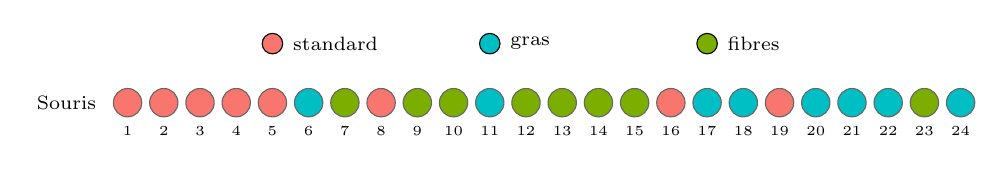
\begin{tikzpicture}[x=4.6mm]
  \foreach \k/\r in {1/grA,2/grA,3/grA,4/grA,5/grA,6/grB,7/grC,8/grA,9/grC,10/grC,
    11/grB,12/grC,13/grC,14/grC,15/grC,16/grA,17/grB,18/grB,19/grA,20/grB,
    21/grB,22/grB,23/grC,24/grB}{
    \draw[black!60, fill=\r] (\k,0) circle (1.8mm);
    \node[font=\tiny, below] at (\k,-0.18) {\k};
  }
  \node[font=\scriptsize, anchor=east] at (0.4,0) {Souris};
  \foreach \x/\c/\t in {5/grA/standard, 11/grB/gras, 17/grC/fibres}{
    \draw[fill=\c] (\x,0.75) circle (1.3mm);
    \node[font=\scriptsize, anchor=west] at (\x+0.3,0.75) {\t};
  }
\end{tikzpicture}
\end{center}

\vspace{-2mm}
{\small Tirage au hasard en R (8 souris par régime):}
\begin{Verbatim}[fontsize=\tiny]
> set.seed(1920)
> sample(rep(c("standard", "gras", "fibres"), each = 8))
 [1] "standard" "standard" "standard" "standard" "standard" "gras"
 [7] "fibres"   "standard" "fibres"   "fibres"   "gras"     "fibres"
[13] "fibres"   "fibres"   "fibres"   "standard" "gras"     "gras"
[19] "standard" "gras"     "gras"     "gras"     "fibres"   "gras"
\end{Verbatim}

\vspace{-2mm}
{\scriptsize Dans une étude observationnelle, on obtient plutôt $I$ échantillons
indépendants en tirant au hasard $n_i$ unités dans chacune des $I$ populations.}

\end{frame}

\begin{frame}[plain,t]
  \centerline{\LARGE\bfseries\alert{QUIZ !}}

  \medskip
  Une agronome compare 4 engrais (A, B, C, D) sur la croissance de plants de
  tomate. Elle dispose de 24 plants, chacun dans son pot. Elle tire au hasard
  6 pots pour chaque engrais et mesure la hauteur des plants (cm) après 6 semaines.

  \medskip
  Identifiez:
  \begin{itemize}\itemsep 0.9cm
    \item la variable réponse;
    \item le facteur et ses niveaux;
    \item l'unité expérimentale;
    \item s'agit-il d'une expérience ou d'une étude observationnelle?
  \end{itemize}
\end{frame}

\begin{frame}[plain,t]
  \centerline{\LARGE\bfseries\alert{QUIZ !}}

  \medskip
  \begin{enumerate}\itemsep 1.4cm
    \item Un biologiste compare la croissance de truites élevées à 3 températures
    de l'eau. Il dispose de 6 bassins (2 par température, tirés au hasard) contenant
    chacun 15 truites. Il mesure la croissance de chaque truite.
    \begin{itemize}
      \item Quelle est l'unité expérimentale?
      \item Combien de répétitions y a-t-il par traitement?
    \end{itemize}
    \item Une écologiste compare la masse moyenne de souris sylvestres capturées
    dans 3 habitats (forêt, champ, milieu périurbain).
    \begin{itemize}
      \item Expérience ou étude observationnelle?
      \item Peut-elle conclure que l'habitat \alert{cause} les différences de masse?
    \end{itemize}
  \end{enumerate}
\end{frame}

%-------------------------------------------------------------------------------
\section{L'idée de l'ANOVA}
%-------------------------------------------------------------------------------

\begin{frame}[t]{ANOVA: décomposition de la variance}

L'analyse de la variance consiste à identifier et à comparer les
\alert{sources de variation} d'une variable:

\medskip

\begin{itemize}\itemsep3mm
  \item<2-> la variabilité \alert{inter-traitements}, entre les moyennes des
  échantillons, que l'on associe au \textbf{facteur} (la caractéristique qui
  distingue les groupes à l'étude);
  \item<3-> la variabilité \alert{intra-traitement}, entre les observations d'un
  même échantillon, que l'on associe à l'\textbf{erreur échantillonnale}
  (non expliquée par le modèle).
\end{itemize}

\end{frame}

\begin{frame}[t]{Comparons deux scénarios}

\begin{columns}[T]
\begin{column}{0.45\textwidth}
\vspace{5mm}
\begin{tabular}{lcc}
\toprule
Moyennes & Scénario 1 & Scénario 2\\
\midrule
Traitement A & 15,32 & 15,32\\
Traitement B & 9,61 & 9,61\\
\bottomrule
\end{tabular}

\bigskip
\uncover<2->{Les moyennes sont \alert{identiques} dans les deux scénarios.
Mais la dispersion à l'intérieur des groupes, elle, ne l'est pas\ldots}
\end{column}
\begin{column}{0.5\textwidth}
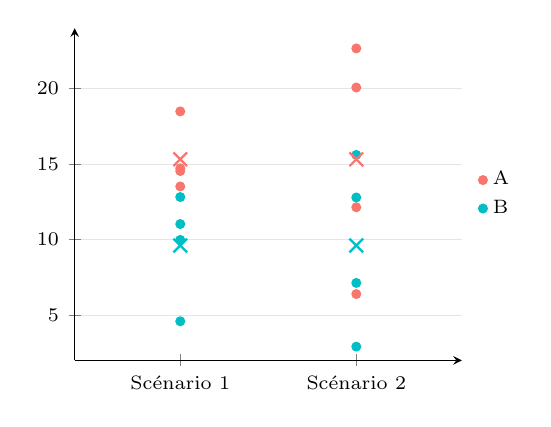
\begin{tikzpicture}
\begin{axis}[pointsANOVA, width=6.5cm, height=5.8cm,
  xtick={1,2}, xticklabels={Scénario 1, Scénario 2},
  legend style={font=\scriptsize, draw=none, at={(1.02,0.5)}, anchor=west},
  legend cell align=left]
  % Scénario 1
  \addplot[only marks, mark=*, mark size=1.6pt, grA] coordinates
    {(1,14.72) (1,13.52) (1,14.54) (1,18.49)};
  \addplot[only marks, mark=*, mark size=1.6pt, grB] coordinates
    {(1,9.98) (1,4.59) (1,12.82) (1,11.03)};
  % Scénario 2
  \addplot[only marks, mark=*, mark size=1.6pt, grA, forget plot] coordinates
    {(2,6.3925) (2,12.1425) (2,20.0725) (2,22.6625)};
  \addplot[only marks, mark=*, mark size=1.6pt, grB, forget plot] coordinates
    {(2,12.79) (2,2.91) (2,7.13) (2,15.61)};
  % Moyennes
  \addplot[only marks, mark=x, mark size=3.5pt, thick, grA, forget plot]
    coordinates {(1,15.32) (2,15.32)};
  \addplot[only marks, mark=x, mark size=3.5pt, thick, grB, forget plot]
    coordinates {(1,9.61) (2,9.61)};
  \legend{A, B}
\end{axis}
\end{tikzpicture}

{\scriptsize $\times$ : moyenne du groupe}
\end{column}
\end{columns}

\end{frame}

% --- Scénario 1 -----------------------------------------------------------------
\begin{frame}[t]{Scénario 1: décomposition de la variance}

\begin{center}
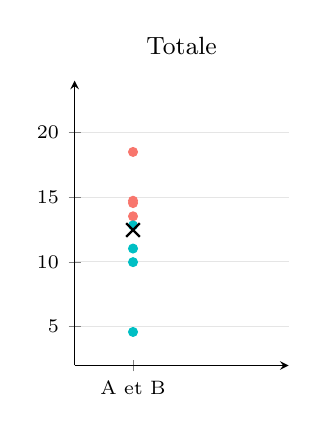
\begin{tikzpicture}
\begin{axis}[pointsANOVA, title=Totale, xtick={1}, xticklabels={A et B}]
  \addplot[only marks, mark=*, mark size=1.6pt, grA] coordinates
    {(1,14.72) (1,13.52) (1,14.54) (1,18.49)};
  \addplot[only marks, mark=*, mark size=1.6pt, grB] coordinates
    {(1,9.98) (1,4.59) (1,12.82) (1,11.03)};
  \addplot[only marks, mark=x, mark size=3.5pt, thick, black] coordinates {(1,12.46)};
\end{axis}
\end{tikzpicture}
\hspace{2mm}
\uncover<2->{%
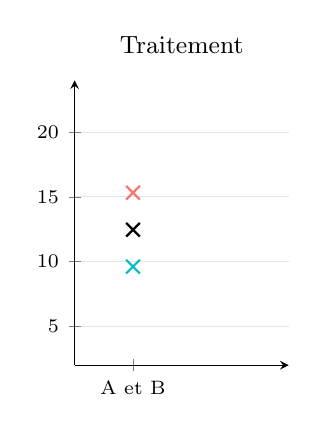
\begin{tikzpicture}
\begin{axis}[pointsANOVA, title=Traitement, xtick={1}, xticklabels={A et B}]
  \addplot[only marks, mark=x, mark size=3.5pt, thick, grA] coordinates {(1,15.32)};
  \addplot[only marks, mark=x, mark size=3.5pt, thick, grB] coordinates {(1,9.61)};
  \addplot[only marks, mark=x, mark size=3.5pt, thick, black] coordinates {(1,12.46)};
\end{axis}
\end{tikzpicture}}
\hspace{2mm}
\uncover<3->{%
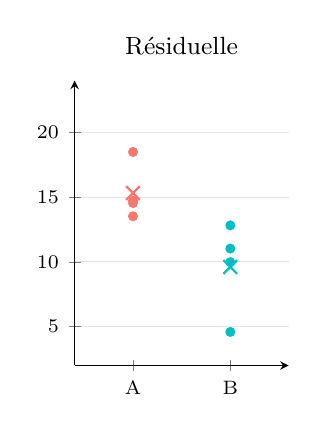
\begin{tikzpicture}
\begin{axis}[pointsANOVA, title=Résiduelle, xtick={1,2}, xticklabels={A, B}]
  \addplot[only marks, mark=*, mark size=1.6pt, grA] coordinates
    {(1,14.72) (1,13.52) (1,14.54) (1,18.49)};
  \addplot[only marks, mark=*, mark size=1.6pt, grB] coordinates
    {(2,9.98) (2,4.59) (2,12.82) (2,11.03)};
  \addplot[only marks, mark=x, mark size=3.5pt, thick, grA] coordinates {(1,15.32)};
  \addplot[only marks, mark=x, mark size=3.5pt, thick, grB] coordinates {(2,9.61)};
\end{axis}
\end{tikzpicture}}
\end{center}

\end{frame}

\begin{frame}[fragile,t]{Scénario 1: table d'analyse de la variance}

\vspace{1cm}
\begin{Verbatim}[fontsize=\small]
           Df Sum Sq Mean Sq F value Pr(>F)
Traitement  1  65.27   65.27   7.543 0.0334 *
Residuals   6  51.91    8.65
---
Signif. codes:  0 '***' 0.001 '**' 0.01 '*' 0.05 '.' 0.1 ' ' 1
\end{Verbatim}

\bigskip
\uncover<2->{La variabilité \alert{entre} les traitements (65,27) est grande
par rapport à la variabilité \alert{à l'intérieur} des traitements (8,65).}

\end{frame}

% --- Scénario 2 -----------------------------------------------------------------
\begin{frame}[t]{Scénario 2: décomposition de la variance}

\begin{center}
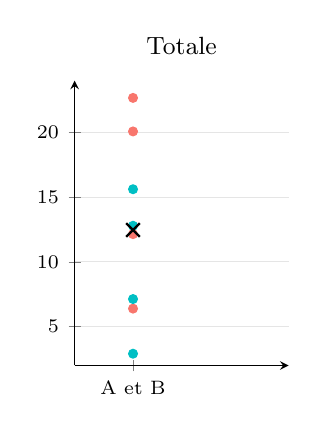
\begin{tikzpicture}
\begin{axis}[pointsANOVA, title=Totale, xtick={1}, xticklabels={A et B}]
  \addplot[only marks, mark=*, mark size=1.6pt, grA] coordinates
    {(1,6.3925) (1,12.1425) (1,20.0725) (1,22.6625)};
  \addplot[only marks, mark=*, mark size=1.6pt, grB] coordinates
    {(1,12.79) (1,2.91) (1,7.13) (1,15.61)};
  \addplot[only marks, mark=x, mark size=3.5pt, thick, black] coordinates {(1,12.46)};
\end{axis}
\end{tikzpicture}
\hspace{2mm}
\uncover<2->{%
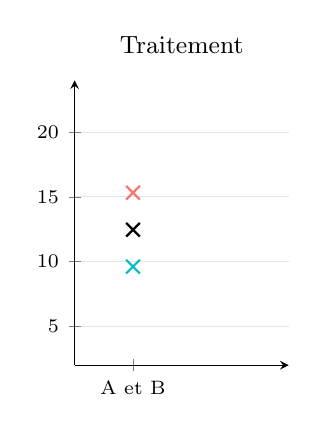
\begin{tikzpicture}
\begin{axis}[pointsANOVA, title=Traitement, xtick={1}, xticklabels={A et B}]
  \addplot[only marks, mark=x, mark size=3.5pt, thick, grA] coordinates {(1,15.32)};
  \addplot[only marks, mark=x, mark size=3.5pt, thick, grB] coordinates {(1,9.61)};
  \addplot[only marks, mark=x, mark size=3.5pt, thick, black] coordinates {(1,12.46)};
\end{axis}
\end{tikzpicture}}
\hspace{2mm}
\uncover<3->{%
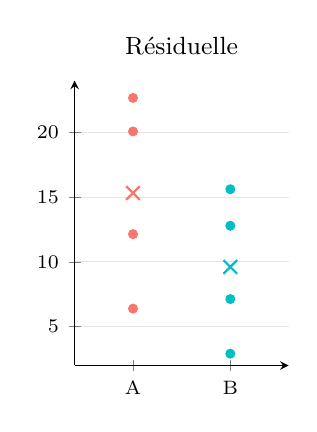
\begin{tikzpicture}
\begin{axis}[pointsANOVA, title=Résiduelle, xtick={1,2}, xticklabels={A, B}]
  \addplot[only marks, mark=*, mark size=1.6pt, grA] coordinates
    {(1,6.3925) (1,12.1425) (1,20.0725) (1,22.6625)};
  \addplot[only marks, mark=*, mark size=1.6pt, grB] coordinates
    {(2,12.79) (2,2.91) (2,7.13) (2,15.61)};
  \addplot[only marks, mark=x, mark size=3.5pt, thick, grA] coordinates {(1,15.32)};
  \addplot[only marks, mark=x, mark size=3.5pt, thick, grB] coordinates {(2,9.61)};
\end{axis}
\end{tikzpicture}}
\end{center}

\end{frame}

\begin{frame}[fragile,t]{Scénario 2: table d'analyse de la variance}

\vspace{1cm}
\begin{Verbatim}[fontsize=\small]
           Df Sum Sq Mean Sq F value Pr(>F)
Traitement  1  65.15   65.15   1.484  0.269
Residuals   6 263.45   43.91
\end{Verbatim}

\bigskip
\uncover<2->{Même écart entre les moyennes, mais la variabilité
\alert{à l'intérieur} des traitements est maintenant beaucoup plus grande:
on ne peut plus conclure à une différence entre A et B.}

\end{frame}

%-------------------------------------------------------------------------------
\section{Mathématique de l'ANOVA}
%-------------------------------------------------------------------------------

\begin{frame}[t]{Cadre}

\textbf{But:} comparer les moyennes $\mu_1,\ldots,\mu_I$ d'une variable $Y$
dans $I$ populations.

\bigskip

\begin{itemize}\itemsep2mm
  \item $Y_{11}, Y_{12}, \ldots, Y_{1n_1}$ sont issues d'une population $N(\mu_1,\sigma^2)$;
  \item $Y_{21}, Y_{22}, \ldots, Y_{2n_2}$ sont issues d'une population $N(\mu_2,\sigma^2)$;
  \item[] $\qquad\vdots$
  \item $Y_{I1}, Y_{I2}, \ldots, Y_{In_I}$ sont issues d'une population $N(\mu_I,\sigma^2)$.
\end{itemize}

\bigskip
\uncover<2->{On note $N=n_1+n_2+\cdots+n_I$ le nombre total d'observations.}

\end{frame}

\begin{frame}[t]{Notation pour les sommes et les moyennes}

\small
$y_{ij}$ = $j$\textsuperscript{e} observation du groupe (traitement) $i$.
Le symbole $\bullet$ remplace un indice sur lequel on a \alert{sommé};
la barre indique une \alert{moyenne}.

\begin{Boite}{Notation}
\vspace{-2mm}
\begin{align*}
y_{i\bullet} &= \sum_{j=1}^{n_i} y_{ij} \ \text{(somme du groupe $i$)},
&
\overline{y}_{i\bullet} &= \frac{y_{i\bullet}}{n_i} \ \text{(moyenne du groupe $i$)},\\
y_{\bullet\bullet} &= \sum_{i=1}^{I}\sum_{j=1}^{n_i} y_{ij} \ \text{(somme totale)},
&
\overline{y}_{\bullet\bullet} &= \frac{y_{\bullet\bullet}}{N} \ \text{(moyenne globale)}.
\end{align*}
\end{Boite}

\uncover<2->{
\small
\underline{Scénario 1} (A = groupe 1, B = groupe 2; $n_1=n_2=4$, $N=8$):\\[1mm]
$y_{1\bullet}=14{,}72+13{,}52+14{,}54+18{,}49=61{,}27$ et
$\overline{y}_{1\bullet}=61{,}27/4=15{,}32$;\\
$y_{2\bullet}=38{,}42$ et $\overline{y}_{2\bullet}=9{,}61$;\quad
$y_{\bullet\bullet}=99{,}69$ et $\overline{y}_{\bullet\bullet}=99{,}69/8=12{,}46$.}

\end{frame}

\begin{frame}[t]{Hypothèses à confronter}

\vspace{1cm}
\begin{Boite}{Hypothèses de l'ANOVA à un facteur}
\begin{align*}
H_0 &: \mu_1 = \mu_2 = \cdots = \mu_I\\[2mm]
H_1 &: \text{au moins 2 moyennes diffèrent}
\end{align*}
\end{Boite}

\end{frame}

\begin{frame}[t]{Le modèle à un facteur}

\begin{Boite}{Modèle}
\[
Y_{ij} = \mu_i + \varepsilon_{ij}, \qquad Y_{ij}\sim N(\mu_i,\sigma^2),
\qquad i=1,\ldots,I,\ j=1,\ldots,n_i
\]
\end{Boite}

\begin{itemize}\itemsep1mm
  \item $\mu_i = $
  \item $\varepsilon_{ij} = $
\end{itemize}

\medskip
\underline{Estimation des paramètres:}

\begin{itemize}\itemsep1mm
  \item $\mu_i$ estimé par
  \item $\mu$ estimé par
  \item $\sigma^2$ estimé par
\end{itemize}

\end{frame}

\begin{frame}[t]{Loi de $Y_{ij}$ sous $H_0$ et sous $H_1$}

\small
On peut écrire $\mu_i=\mu+\tau_i$, où $\mu$ est la moyenne globale et
$\tau_i=\mu_i-\mu$ est l'\alert{effet} du traitement $i$.
Alors $H_0: \mu_1=\cdots=\mu_I \iff H_0: \tau_1=\cdots=\tau_I=0$.

\begin{center}
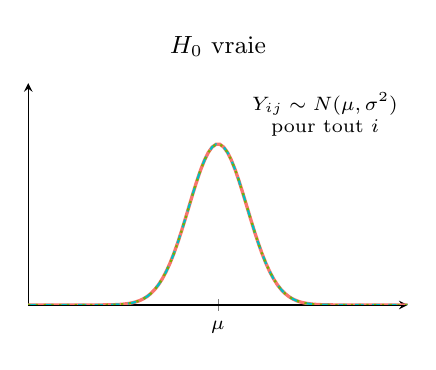
\begin{tikzpicture}
\begin{axis}[width=6.4cm, height=4.4cm, axis lines=left, xmin=0, xmax=13,
  ymin=0, ymax=0.55, ytick=\empty, xtick={6.5}, xticklabels={$\mu$},
  tick label style={font=\scriptsize}, title={$H_0$ vraie}, title style={font=\small},
  domain=0:13, samples=100]
  \addplot[grA, very thick] {exp(-((x-6.5)^2)/2)/sqrt(2*pi)};
  \addplot[grB, thick, dashed] {exp(-((x-6.5)^2)/2)/sqrt(2*pi)};
  \addplot[grC, thick, dotted] {exp(-((x-6.5)^2)/2)/sqrt(2*pi)};
  \node[font=\scriptsize, align=center, anchor=north east] at (axis cs:13,0.55)
    {$Y_{ij}\sim N(\mu,\sigma^2)$\\pour tout $i$};
\end{axis}
\end{tikzpicture}
\hspace{2mm}
\uncover<2->{%
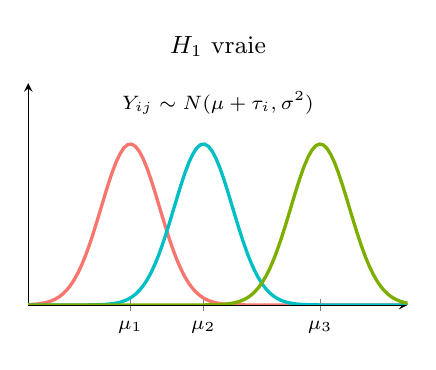
\begin{tikzpicture}
\begin{axis}[width=6.4cm, height=4.4cm, axis lines=left, xmin=0, xmax=13,
  ymin=0, ymax=0.55, ytick=\empty, xtick={3.5,6,10}, xticklabels={$\mu_1$,$\mu_2$,$\mu_3$},
  tick label style={font=\scriptsize}, title={$H_1$ vraie}, title style={font=\small},
  domain=0:13, samples=100]
  \addplot[grA, very thick] {exp(-((x-3.5)^2)/2)/sqrt(2*pi)};
  \addplot[grB, very thick] {exp(-((x-6)^2)/2)/sqrt(2*pi)};
  \addplot[grC, very thick] {exp(-((x-10)^2)/2)/sqrt(2*pi)};
  \node[font=\scriptsize, align=center] at (axis cs:6.5,0.5)
    {$Y_{ij}\sim N(\mu+\tau_i,\sigma^2)$};
\end{axis}
\end{tikzpicture}}
\end{center}

\uncover<2->{Sous $H_0$, les $I$ groupes proviennent de la \alert{même} loi normale.
Sous $H_1$, les lois ont la \alert{même forme} (même $\sigma^2$), mais au moins deux
sont \alert{décalées}.}

\end{frame}

\begin{frame}[t]{Décomposition de la variance}

\begin{Boite}{Décomposition des sommes de carrés}
\vspace{-3mm}
\begin{align*}
SST &= SST_R + SSE\\
\sum_{i=1}^{I}\sum_{j=1}^{n_i}(y_{ij}-\overline{y}_{\bullet\bullet})^2
&= \sum_{i=1}^{I} n_i(\overline{y}_{i\bullet}-\overline{y}_{\bullet\bullet})^2
+ \sum_{i=1}^{I}\sum_{j=1}^{n_i}(y_{ij}-\overline{y}_{i\bullet})^2
\end{align*}
\end{Boite}

\begin{center}
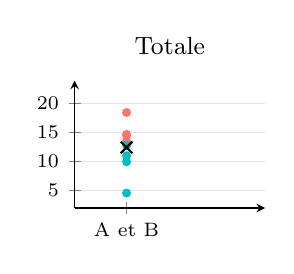
\begin{tikzpicture}
\begin{axis}[pointsANOVA, height=3.2cm, width=4cm, title=Totale, xtick={1}, xticklabels={A et B}]
  \addplot[only marks, mark=*, mark size=1.4pt, grA] coordinates
    {(1,14.72) (1,13.52) (1,14.54) (1,18.49)};
  \addplot[only marks, mark=*, mark size=1.4pt, grB] coordinates
    {(1,9.98) (1,4.59) (1,12.82) (1,11.03)};
  \addplot[only marks, mark=x, mark size=3pt, thick, black] coordinates {(1,12.46)};
\end{axis}
\end{tikzpicture}
\hspace{2mm}
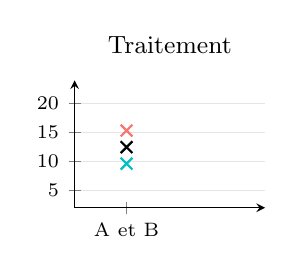
\begin{tikzpicture}
\begin{axis}[pointsANOVA, height=3.2cm, width=4cm, title=Traitement, xtick={1}, xticklabels={A et B}]
  \addplot[only marks, mark=x, mark size=3pt, thick, grA] coordinates {(1,15.32)};
  \addplot[only marks, mark=x, mark size=3pt, thick, grB] coordinates {(1,9.61)};
  \addplot[only marks, mark=x, mark size=3pt, thick, black] coordinates {(1,12.46)};
\end{axis}
\end{tikzpicture}
\hspace{2mm}
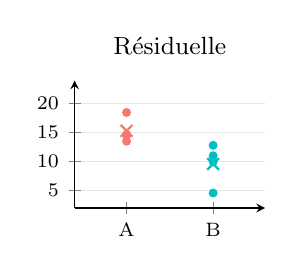
\begin{tikzpicture}
\begin{axis}[pointsANOVA, height=3.2cm, width=4cm, title=Résiduelle, xtick={1,2}, xticklabels={A, B}]
  \addplot[only marks, mark=*, mark size=1.4pt, grA] coordinates
    {(1,14.72) (1,13.52) (1,14.54) (1,18.49)};
  \addplot[only marks, mark=*, mark size=1.4pt, grB] coordinates
    {(2,9.98) (2,4.59) (2,12.82) (2,11.03)};
  \addplot[only marks, mark=x, mark size=3pt, thick, grA] coordinates {(1,15.32)};
  \addplot[only marks, mark=x, mark size=3pt, thick, grB] coordinates {(2,9.61)};
\end{axis}
\end{tikzpicture}
\end{center}

\end{frame}

\begin{frame}[plain,t]
  \centerline{\LARGE\bfseries\alert{QUIZ !}}

  \medskip
  Deux expériences ont obtenu les mêmes \alert{variances} échantillonnales
  (même dispersion dans chaque groupe):

  \begin{center}
  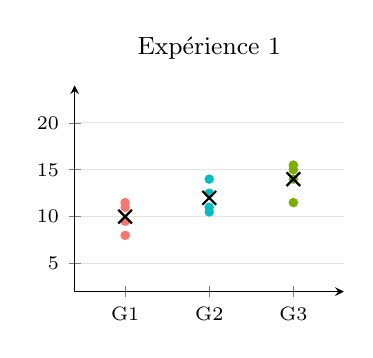
\begin{tikzpicture}
  \begin{axis}[pointsANOVA, width=5cm, height=4.2cm, xmin=0.4, xmax=3.6,
    xtick={1,2,3}, xticklabels={G1, G2, G3}, title={Expérience 1}]
    \addplot[only marks, mark=*, mark size=1.5pt, grA] coordinates {(1,8) (1,9.5) (1,11) (1,11.5)};
    \addplot[only marks, mark=*, mark size=1.5pt, grB] coordinates {(2,10.5) (2,11) (2,12.5) (2,14)};
    \addplot[only marks, mark=*, mark size=1.5pt, grC] coordinates {(3,11.5) (3,14) (3,15) (3,15.5)};
    \addplot[only marks, mark=x, mark size=3.5pt, thick, black] coordinates {(1,10) (2,12) (3,14)};
  \end{axis}
  \end{tikzpicture}
  \hspace{6mm}
  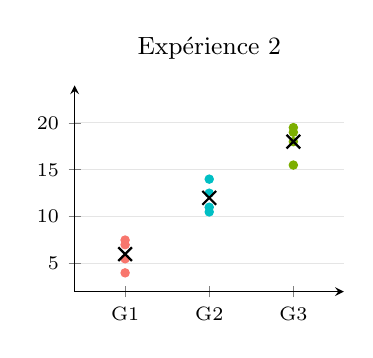
\begin{tikzpicture}
  \begin{axis}[pointsANOVA, width=5cm, height=4.2cm, xmin=0.4, xmax=3.6,
    xtick={1,2,3}, xticklabels={G1, G2, G3}, title={Expérience 2}]
    \addplot[only marks, mark=*, mark size=1.5pt, grA] coordinates {(1,4) (1,5.5) (1,7) (1,7.5)};
    \addplot[only marks, mark=*, mark size=1.5pt, grB] coordinates {(2,10.5) (2,11) (2,12.5) (2,14)};
    \addplot[only marks, mark=*, mark size=1.5pt, grC] coordinates {(3,15.5) (3,18) (3,19) (3,19.5)};
    \addplot[only marks, mark=x, mark size=3.5pt, thick, black] coordinates {(1,6) (2,12) (3,18)};
  \end{axis}
  \end{tikzpicture}
  \end{center}

  \begin{itemize}\itemsep 0.6cm
    \item Quelle expérience a le plus grand $SST_R$? le plus grand $SSE$? le plus grand $SST$?
    \item Et pour les scénarios 1 et 2 vus plus tôt (mêmes \alert{moyennes})?
  \end{itemize}
\end{frame}

\begin{frame}[t]{Table d'ANOVA}

\vspace{5mm}
\begin{center}
\renewcommand{\arraystretch}{2.3}
\begin{tabular}{lcccc}
\toprule
Source de variation & Somme de carrés & d.l. & Carrés moyens & $F_{obs}$\\
\midrule
Traitements (inter-trt) & $SST_R$ & $I-1$ & $MST_R=\dfrac{SST_R}{I-1}$ & $\dfrac{MST_R}{MSE}$\\
Erreur (intra-trt)     & $SSE$   & $N-I$ & $MSE=\dfrac{SSE}{N-I}$   & \\
\midrule
Total                  & $SST$   & $N-1$ &                          & \\
\bottomrule
\end{tabular}
\end{center}

\end{frame}

\begin{frame}[t]{Comparer $MST_R$ et $MSE$}

\begin{itemize}\itemsep4mm
  \item S'il n'y a pas de différence entre les traitements ($H_0$ vraie),
  $MST_R$ et $MSE$ sont tous les deux de bons estimateurs de $\sigma^2$.
  \item<2-> Si l'effet des traitements est important, on aura
  \[
  MST_R \gg MSE.
  \]
\end{itemize}

\bigskip
\uncover<3->{\alert{Question:} à partir de quand considère-t-on que $MST_R$ est
vraiment plus grand que $MSE$?}

\end{frame}

\begin{frame}[t]{Pourquoi $F\approx 1$ sous $H_0$? Espérance des carrés moyens}

\begin{Boite}{Espérance des carrés moyens}
On peut montrer que
\[
E(MSE)=\sigma^2
\qquad\text{et}\qquad
E(MST_R)=\sigma^2+\frac{\sum_{i=1}^{I} n_i\tau_i^2}{I-1},
\qquad\text{où } \tau_i=\mu_i-\mu.
\]
\end{Boite}

\small
\begin{itemize}\itemsep1mm
  \item $MSE$ estime toujours $\sigma^2$, que $H_0$ soit vraie ou non.
  \item<2-> Sous $H_0$: tous les $\tau_i=0$ $\Rightarrow$ $E(MST_R)=\sigma^2$
  $\Rightarrow$ $F=MST_R/MSE$ devrait être \alert{proche de 1}.
  \item<2-> Sous $H_1$: au moins un $\tau_i\neq0$ $\Rightarrow$ $E(MST_R)>\sigma^2$
  $\Rightarrow$ $F$ tend à être \alert{plus grand que 1}.
  \item<3-> On rejette donc $H_0$ seulement pour les \alert{grandes} valeurs de $F$.
\end{itemize}

\end{frame}

\begin{frame}[t]{Statistique de Fisher}

\begin{thm}
Si
\begin{itemize}
  \item les observations sont \alert{indépendantes} (dans les groupes et entre les groupes),
  \item les données proviennent d'une distribution \alert{normale},
  \item la \alert{variance est égale} dans chaque groupe,
\end{itemize}
et que $H_0$ est vraie ($\mu_i$ toutes égales), alors
\[
F=\frac{SST_R/(I-1)}{SSE/(N-I)}=\frac{MST_R}{MSE}\sim F_{I-1,\,N-I}.
\]
\end{thm}

\end{frame}

\begin{frame}[t]{Règle de décision}

\begin{Boite}{Test F de l'ANOVA}
On rejette $H_0$ au seuil $\alpha$ si
\[
F_{obs} > F_{I-1,\,N-I;\,\alpha}.
\]
Dans ce cas, on a une valeur-p inférieure à $\alpha$.
\end{Boite}

\begin{center}
\begin{tikzpicture}
\begin{axis}[width=9cm, height=3.7cm, axis lines=left, xmin=0, xmax=6, ymin=0,
  ytick=\empty, xtick={3.89}, xticklabels={$F_{I-1,N-I;\alpha}$},
  tick label style={font=\scriptsize}, domain=0.01:6, samples=120]
  % Densité F(2,12) : f(x) = (1+x/6)^(-7)
  \addplot[draw=none, fill=burntorange, domain=3.89:6] {(1+x/6)^(-7)} \closedcycle;
  \addplot[thick, black] {(1+x/6)^(-7)};
  \node[font=\scriptsize] at (axis cs:4.7,0.12) {aire $=\alpha$};
\end{axis}
\end{tikzpicture}
\end{center}

\end{frame}

\begin{frame}[fragile,t]{Retour au scénario 1}

\begin{columns}[T]
\begin{column}{0.4\textwidth}
\begin{Verbatim}[fontsize=\scriptsize]
     y1   Traitement
1 14.72   A
2 13.52   A
3 14.54   A
4 18.49   A
5  9.98   B
6  4.59   B
7 12.82   B
8 11.03   B
\end{Verbatim}
\end{column}
\begin{column}{0.55\textwidth}
\begin{tabular}{lcc}
\toprule
 & Moyenne & Écart-type\\
\midrule
A & 15,32 & 2,18\\
B & 9,61  & 3,54\\
\bottomrule
\end{tabular}
\end{column}
\end{columns}

\medskip
\begin{Verbatim}[fontsize=\scriptsize]
           Df Sum Sq Mean Sq F value Pr(>F)
Traitement  1  65.27   65.27   7.543 0.0334 *
Residuals   6  51.91    8.65
\end{Verbatim}

\uncover<2->{\small Vérifier: $SST_R = 4(15{,}32-12{,}46)^2+4(9{,}61-12{,}46)^2\approx 65{,}27$
et $SSE = 3(2{,}18^2)+3(3{,}54^2)\approx 51{,}9$.}

\end{frame}

\begin{frame}[plain,t]
  \centerline{\LARGE\bfseries\alert{QUIZ !}}

  \medskip
  Retour aux 4 engrais appliqués à 24 plants de tomate (6 par engrais).
  On obtient $SST_R=84{,}0$ et $SST=224{,}0$. Complétez la table d'ANOVA.

  \begin{center}
  \renewcommand{\arraystretch}{1.5}
  \begin{tabular}{lcccc}
  \toprule
  Source & Somme de carrés & d.l. & Carré moyen & $F_{obs}$\\
  \midrule
  Engrais & $84{,}0$ & \hspace{1cm} & \hspace{1.5cm} & \hspace{1cm}\\
  Erreur  & & & & \\
  \midrule
  Total   & $224{,}0$ & & & \\
  \bottomrule
  \end{tabular}
  \end{center}

  \begin{itemize}\itemsep 0.9cm
    \item Sachant que $F_{3,\,20;\,0{,}05}=3{,}10$, que concluez-vous au seuil de 5\,\%?
    \item Combien vaut l'estimation de $\sigma^2$? Et celle de $\sigma$?
  \end{itemize}
\end{frame}

\begin{frame}[fragile,t]{Aurait-on pu faire un test de Student?}

\underline{ANOVA:}
\begin{Verbatim}[fontsize=\scriptsize]
           Df Sum Sq Mean Sq F value Pr(>F)
Traitement  1  65.27   65.27   7.543 0.0334 *
Residuals   6  51.91    8.65
\end{Verbatim}

\underline{Test de Student:}
\begin{Verbatim}[fontsize=\scriptsize]
        Two Sample t-test
data:  y1 by Traitement
t = 2.7464, df = 6, p-value = 0.03345
alternative hypothesis: true difference in means between group A and group B
  is not equal to 0
95 percent confidence interval:
  0.6230128 10.8019872
sample estimates:
mean in group A mean in group B
        15.3175          9.6050
\end{Verbatim}

\end{frame}

\begin{frame}[t]{Student vs ANOVA}

\begin{itemize}\itemsep8mm
  \item Est-ce un hasard si les valeurs-p sont les mêmes?
  \vspace{2cm}
  \item Pourquoi faire l'ANOVA?
  \vspace{2cm}
\end{itemize}

\end{frame}

\begin{frame}[t]{Exemple: agent de conservation naturel pour la viande}

\small
\underline{Contexte:} agent de conservation à partir de sang de porc
(\href{https://nouvelles.ulaval.ca/recherche/de-residu-a-source-dagents-de-conservation-naturels-0797d4c252cd98ac53f75a256e95624a}{ULaval Nouvelles}).

\begin{itemize}\itemsep2mm
  \item En 2016, environ 30 millions de litres de sang bovin et porcin ont été
  produits au Québec.
  \item Une nouvelle méthode d'extraction (EDUF) permet une plus grande
  concentration de peptides bioactifs.
  \item Selon les chercheurs, ces extraits de sang se sont montrés aussi efficaces
  que le BHT, un additif chimique couramment utilisé par l'industrie alimentaire,
  lors de tests sur du b\oe uf haché.
  \item Nous avons \alert{simulé} des données à partir des moyennes et écarts-types
  de la section 3.6 de l'article.
\end{itemize}

\end{frame}

\begin{frame}[t]{Contexte}

\begin{itemize}\itemsep4mm
  \item On veut comparer l'effet antioxydant de l'\alert{EDUF} (la nouvelle méthode)
  au peptide original nommé \alert{$\alpha$137--141} et à un \alert{contrôle}.
  \item On crée un échantillon de taille 6 pour chaque traitement.
  \item On mesure le \alert{TBARS} (en mg MDA/kg de viande hachée) après 4 jours
  (une mesure de rancissement).
\end{itemize}

\end{frame}

\begin{frame}[t]{Premier réflexe: regarder les données}

\small
Avant toute analyse, on \alert{visualise} les données de chaque groupe
(diagrammes en boîte ou diagrammes en points).

\begin{center}
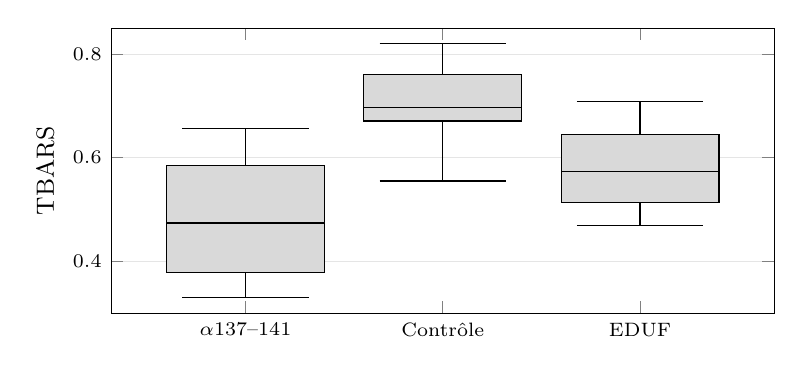
\begin{tikzpicture}
\begin{axis}[width=10cm, height=5.2cm, boxplot/draw direction=y,
  ylabel={TBARS}, xtick={1,2,3},
  xticklabels={$\alpha$137--141, Contrôle, EDUF},
  ymin=0.3, ymax=0.85, tick label style={font=\scriptsize},
  label style={font=\small}, ymajorgrids, grid style={black!10}]
  \addplot+[boxplot prepared={lower whisker=0.33, lower quartile=0.378,
    median=0.474, upper quartile=0.585, upper whisker=0.657},
    black, fill=black!15] coordinates {};
  \addplot+[boxplot prepared={lower whisker=0.555, lower quartile=0.671,
    median=0.697, upper quartile=0.760, upper whisker=0.820},
    black, fill=black!15] coordinates {};
  \addplot+[boxplot prepared={lower whisker=0.47, lower quartile=0.513,
    median=0.574, upper quartile=0.645, upper whisker=0.709},
    black, fill=black!15] coordinates {};
\end{axis}
\end{tikzpicture}
\end{center}

\vspace{-2mm}
\begin{itemize}\itemsep0mm
  \item<2-> Les TBARS moyens semblent-ils différer d'un traitement à l'autre?
  \item<2-> La dispersion est-elle semblable dans les trois groupes? Y a-t-il des valeurs extrêmes?
\end{itemize}

\end{frame}

\begin{frame}[t]{Test ANOVA}

\textbf{1. Hypothèses}

$H_0$: les trois moyennes sont égales

$H_1$: au moins une moyenne est différente d'une autre

\bigskip
\uncover<2->{\textbf{2. Choix du test et définition de la zone de rejet}

Si les données sont distribuées normalement et que les variances sont égales,
on fait une analyse de variance à un facteur.

\medskip
On choisit $\alpha$. On rejette $H_0$ si la valeur-p est inférieure à $\alpha$.
Choisissons arbitrairement $\alpha = 0{,}05$.}

\end{frame}

\begin{frame}[t]{Table d'ANOVA à compléter}

\textbf{3. On fait le test avec un logiciel}

\medskip
On obtient (en partie) la table suivante. Complétez-la.

\vspace{3mm}
\begin{center}
\renewcommand{\arraystretch}{1.8}
\begin{tabular}{lcccc}
\toprule
Source de variation & Somme de carrés & d.l. & Carrés moyens & $F_{obs}$\\
\midrule
Traitements (inter-trt) & \hspace{1.5cm} & \hspace{1cm} & \hspace{2cm} & \hspace{1cm}\\
Erreur (intra-trt)     &          &        & $0{,}0104$ & \\
\midrule
Total                  & $0{,}2971$ &      &            & \\
\bottomrule
\end{tabular}
\end{center}

\end{frame}

\begin{frame}[fragile,t]{Sortie R}

\begin{Verbatim}[fontsize=\small]
           Df Sum Sq Mean Sq F value  Pr(>F)
Traitement  2 0.1412  0.0706   6.791 0.00794 **
Residuals  15 0.1559  0.0104
---
Signif. codes:  0 '***' 0.001 '**' 0.01 '*' 0.05 '.' 0.1 ' ' 1
\end{Verbatim}

\bigskip
\textbf{4. Décision}
\vspace{1.5cm}

\textbf{5. Conclusion}
\vspace{1.5cm}

\end{frame}

\begin{frame}[plain,t]
  \centerline{\LARGE\bfseries\alert{QUIZ !}}

  \medskip
  Lorsque $H_0$ est rejetée dans une ANOVA à un facteur, lesquelles des conclusions
  suivantes sont correctes?
  \begin{itemize}\itemsep 0.45cm
    \item Toutes les moyennes sont égales.
    \item Toutes les moyennes sont différentes.
    \item Au moins deux moyennes sont différentes.
    \item La variable réponse a un effet sur le facteur.
    \item Le facteur a un effet sur la variable réponse.
    \item Le contrôle a un TBARS moyen plus élevé que l'EDUF.
  \end{itemize}
\end{frame}

\begin{frame}[t]{Contrastes}

\begin{itemize}\itemsep8mm
  \item Comment savoir \alert{quelles} moyennes sont différentes? (section 5.8)
  \vspace{1.5cm}
  \item Peut-on simplement faire plusieurs tests de Student 2 à 2?
  \vspace{1.5cm}
\end{itemize}

\end{frame}

\begin{frame}[t]{Le problème des comparaisons multiples}

\small
Chaque test de Student au seuil $\alpha=5\,\%$ a 5\,\% de chances de conclure à
tort à une différence. Plus on fait de tests, plus le risque qu'\alert{au moins un}
d'entre eux donne une fausse alerte augmente (comme acheter plusieurs billets de
loterie!).

\begin{center}
\scriptsize
\renewcommand{\arraystretch}{1.1}
\begin{tabular}{ccc}
\toprule
Groupes ($I$) & Comparaisons 2 à 2 ($m$) & $P(\text{au moins une fausse alerte})\approx 1-0{,}95^{m}$\\
\midrule
3  & 3  & 0,14\\
4  & 6  & 0,26\\
5  & 10 & 0,40\\
10 & 45 & 0,90\\
\bottomrule
\end{tabular}

{\tiny (Approximation qui suppose les tests indépendants.)}
\end{center}

\vspace{-4mm}
\uncover<2->{
\begin{Boite}{Méthode de Tukey}
Compare toutes les paires de moyennes en ajustant les valeurs-p (et les
intervalles de confiance) pour que le \alert{taux d'erreur global} (probabilité
d'au moins une fausse alerte) soit égal à $\alpha$.
\end{Boite}}

\end{frame}

\begin{frame}[fragile,t]{Comparaisons multiples de Tukey}

\begin{Verbatim}[fontsize=\scriptsize]
         Simultaneous Tests for General Linear Hypotheses

Multiple Comparisons of Means: Tukey Contrasts

Fit: aov(formula = TBARS ~ Traitement, data = conservation)

Linear Hypotheses:
                          Estimate Std. Error t value Pr(>|t|)
Controle - a137_141 == 0   0.21658    0.05887   3.679  0.00599 **
EDUF - a137_141 == 0       0.09732    0.05887   1.653  0.25496
EDUF - Controle == 0      -0.11926    0.05887  -2.026  0.14031
---
Signif. codes:  0 '***' 0.001 '**' 0.01 '*' 0.05 '.' 0.1 ' ' 1
(Adjusted p values reported -- single-step method)
\end{Verbatim}

\end{frame}

\begin{frame}[t]{Intervalles de confiance simultanés (Tukey)}

\begin{center}
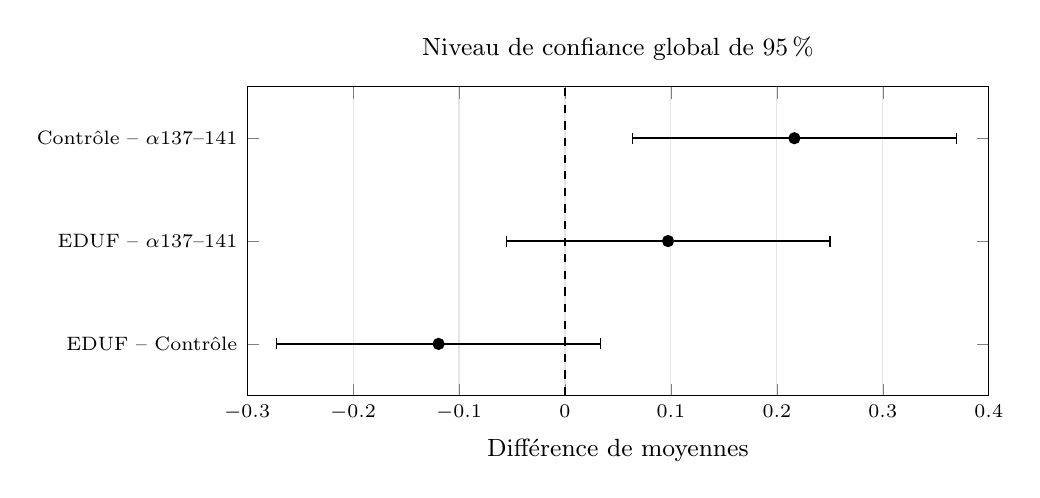
\begin{tikzpicture}
\begin{axis}[width=11cm, height=5.5cm, xmin=-0.3, xmax=0.4,
  ymin=0.5, ymax=3.5, ytick={1,2,3},
  yticklabels={EDUF -- Contrôle, EDUF -- $\alpha$137--141, Contrôle -- $\alpha$137--141},
  xlabel={Différence de moyennes}, title={Niveau de confiance global de 95\,\%},
  tick label style={font=\scriptsize}, label style={font=\small},
  title style={font=\small}, xmajorgrids, grid style={black!10}]
  \draw[dashed] (axis cs:0,0.5) -- (axis cs:0,3.5);
  \addplot[only marks, mark=*, black,
    error bars/.cd, x dir=both, x explicit, error bar style={thick}]
    coordinates {
      (-0.11926,1) +- (0.1529,0)
      (0.09732,2)  +- (0.1529,0)
      (0.21658,3)  +- (0.1529,0)
    };
\end{axis}
\end{tikzpicture}
\end{center}

\uncover<2->{\small Seul l'intervalle Contrôle -- $\alpha$137--141 ne contient pas 0.}

\end{frame}

%-------------------------------------------------------------------------------
\section{Vérification des postulats}
%-------------------------------------------------------------------------------

\begin{frame}[t]{Indépendance des observations: structure de l'expérience}

\vspace{1cm}
\begin{itemize}\itemsep5mm
  \item Y a-t-il des liens entre les observations d'un même traitement?
  De traitements différents?
  \item A-t-on pris plusieurs mesures sur une même unité expérimentale?
\end{itemize}

\end{frame}

\begin{frame}[t]{Homogénéité des variances: test de Bartlett}

On veut tester les hypothèses
\begin{align*}
H_0 &: \sigma_1^2=\sigma_2^2=\cdots=\sigma_I^2\\
H_1 &: \text{au moins 2 de ces variances sont inégales}
\end{align*}

On utilise une statistique $B$ (appelée \texttt{K-squared} dans R):
\begin{itemize}\itemsep2mm
  \item<2-> si $H_0$ est vraie, $B$ suit une loi $\chi^2_{I-1}$;
  \item<3-> si $H_1$ est vraie, $B$ prendra des valeurs plus élevées que celles
  attendues sous la $\chi^2_{I-1}$;
  \item<4-> alors, au seuil $\alpha$, on rejette l'égalité des variances si\ldots
\end{itemize}

\end{frame}

\begin{frame}[fragile,t]{Exemple}

\vspace{1cm}
\begin{Verbatim}[fontsize=\small]
        Bartlett test of homogeneity of variances

data:  TBARS by Traitement
Bartlett's K-squared = 0.74383, df = 2, p-value = 0.6894
\end{Verbatim}

\bigskip
\uncover<2->{Conclusion?}

\end{frame}

\begin{frame}[t]{Normalité des observations: analyse des résidus}

Rappel du modèle:
\[
Y_{ij}=\mu_i+\varepsilon_{ij}
\]
Puisque $Y_{ij}\sim N(\mu_i,\sigma^2)$, il suit que $\varepsilon_{ij}\sim N(0,\sigma^2)$.

\medskip
\begin{Boite}{Résidus}
Les erreurs échantillonnales $\varepsilon_{ij}$ sont estimées par les
\alert{résidus} du modèle:
\[
\hat\varepsilon_{ij}=y_{ij}-\overline{y}_{i\bullet}.
\]
\end{Boite}

Au lieu d'analyser directement les observations, nous analyserons les résidus.

\end{frame}

\begin{frame}[fragile,t]{Test de normalité sur les résidus}

\vspace{1cm}
\begin{Verbatim}[fontsize=\small]
        Shapiro-Wilk normality test

data:  AnovaModel.3$residuals
W = 0.97151, p-value = 0.8255
\end{Verbatim}

\bigskip
\uncover<2->{Conclusion?}

\end{frame}

\begin{frame}[t]{Réponses aux exemples}

\scriptsize
\begin{itemize}\itemsep1mm
  \item \textbf{Quiz (tomates):} variable réponse = hauteur des plants (cm) après
  6 semaines; facteur = engrais, à 4 niveaux (A, B, C, D); unité expérimentale = un
  plant (pot); c'est une \alert{expérience} (engrais attribués au hasard): devis
  complètement aléatoire avec $n_i=6$.
  \item \textbf{Quiz (truites):} le traitement (température) est appliqué au
  \alert{bassin}: l'unité expérimentale est le bassin, et il n'y a que \alert{2
  répétitions} par température (et non 30). Les truites d'un même bassin ne sont pas
  indépendantes.
  \item \textbf{Quiz (souris sylvestres):} étude observationnelle; on ne peut pas
  conclure à un lien de cause à effet (l'habitat est confondu avec la nourriture
  disponible, les prédateurs, la densité de population\ldots).
  \item \textbf{Modèle:} $\mu_i$ est la moyenne de la population $i$;
  $\varepsilon_{ij}=Y_{ij}-\mu_i$ est l'erreur aléatoire, $\varepsilon_{ij}\sim N(0,\sigma^2)$.
  On estime $\mu_i$ par $\overline{y}_{i\bullet}$, $\mu$ par $\overline{y}_{\bullet\bullet}$
  et $\sigma^2$ par $MSE$.
  \item \textbf{Quiz (même variance):} l'expérience 2 a le plus grand $SST_R$
  ($288$ contre $32$) et le plus grand $SST$ ($312{,}5$ contre $56{,}5$); les $SSE$ sont
  égales ($24{,}5$). Scénarios 1 et 2: $SST_R$ presque égales ($65{,}27$ et $65{,}15$),
  mais $SSE$ ($51{,}91$ contre $263{,}45$) et $SST$ ($117{,}18$ contre $328{,}60$) plus
  grandes dans le scénario 2.
  \item \textbf{Quiz (table des engrais):} $SSE=224-84=140$; d.l.\ $3$, $20$ et $23$;
  $MST_R=28$, $MSE=7$; $F_{obs}=4{,}00>3{,}10$: on rejette $H_0$ (valeur-p $=0{,}022$);
  au moins deux engrais mènent à des hauteurs moyennes différentes.
  $\hat\sigma^2=MSE=7$, $\hat\sigma=\sqrt{7}=2{,}65$\,cm.
\end{itemize}

\end{frame}

\begin{frame}[t]{Réponses aux exemples (suite)}

\scriptsize
\begin{itemize}\itemsep1mm
  \item \textbf{Student vs ANOVA:} avec deux groupes, $F_{obs}=t_{obs}^2$
  ($2{,}7464^2\approx7{,}543$) et $F_{1,\nu}=t_\nu^2$: les deux tests sont équivalents.
  L'ANOVA permet de comparer plus de deux groupes en un seul test.
  \item \textbf{Regarder les données (TBARS):} le contrôle semble avoir un TBARS plus
  élevé que les deux autres traitements; les dispersions sont semblables et on ne voit
  pas de valeur extrême.
  \item \textbf{Table à compléter:} $SST_R=0{,}1412$, $SSE=0{,}1559$, d.l.\ $2$, $15$,
  $17$; $MST_R=0{,}0706$; $F_{obs}=6{,}79$.
  \item \textbf{Décision:} valeur-p $=0{,}008<0{,}05$, on rejette $H_0$.
  \textbf{Conclusion:} au seuil de 5\,\%, au moins un traitement a un TBARS moyen
  différent des autres.
  \item \textbf{Quiz ($H_0$ rejetée):} seules « Au moins deux moyennes sont
  différentes » et « Le facteur a un effet sur la variable réponse » sont correctes.
  Le test $F$ ne dit pas \alert{quelles} moyennes diffèrent (d'ailleurs, Tukey ne
  détecte pas de différence significative entre le contrôle et l'EDUF, $p=0{,}14$).
  \item \textbf{Plusieurs tests 2 à 2:} le risque global d'erreur de type I augmente
  avec le nombre de comparaisons; d'où les comparaisons multiples (Tukey).
  \item \textbf{Bartlett:} valeur-p $=0{,}69$, on ne rejette pas l'égalité des
  variances. On rejette si $B>\chi^2_{I-1;\,\alpha}$.
  \item \textbf{Shapiro-Wilk:} valeur-p $=0{,}83$, pas d'évidence contre la normalité.
\end{itemize}

\end{frame}

\end{document}
